\documentclass[11 pt]{article}

\setlength{\oddsidemargin}{-.45in}
%\setlength{\evensidemargin}{-.5in}
\setlength{\textwidth}{7.25in}
\setlength{\topmargin}{-0.95in}
\setlength{\textheight}{10.2in}

\usepackage{graphics}
\usepackage{latexsym}
\usepackage{amsfonts}
\usepackage{amsmath}
\usepackage{amsthm}
\usepackage{epstopdf}
%\usepackage{multicol}
%\usepackage{wrapfig}
\pagestyle{empty}

\usepackage[T1]{fontenc}
\usepackage{baskervald}
\usepackage[bigdelims,vvarbb]{newtxmath} 

\newcommand{\ds}{\ensuremath{\displaystyle}}
\newcommand{\tr}{\vspace{0.5in}}
\newcommand{\lr}{\vspace{1.0in}}
\newcommand{\mr}{\vspace{2.0in}}
\newcommand{\br}{\vspace{3.0in}}

\newcommand{\ps}{Problem Set~}
\newcommand{\vi}{\ensuremath{\mathbf{i}}}
\newcommand{\vj}{\ensuremath{\mathbf{j}}}
\newcommand{\vk}{\ensuremath{\mathbf{k}}}
\newcommand{\vr}{\ensuremath{\mathbf{r}}}
\newcommand{\vecv}{\ensuremath{\mathbf{v}}}
\newcommand{\vu}{\ensuremath{\mathbf{u}}}
\newcommand{\va}{\ensuremath{\mathbf{a}}}
\newcommand{\vs}{\ensuremath{\mathbf{s}}}
\newcommand{\ve}{\ensuremath{\mathbf{e}}}
\newcommand{\vx}{\ensuremath{\mathbf{x}}}
\newcommand{\vc}{\ensuremath{\mathbf{c}}}
\newcommand{\vb}{\ensuremath{\mathbf{b}}}

\usepackage{hyperref} 
\hypersetup{colorlinks=true, linkcolor=blue,  anchorcolor=blue,  
citecolor=blue, filecolor=blue, menucolor=blue, pagecolor=blue,  
urlcolor=blue,pdftitle={MTH 202 Checkpoint}}

\usepackage{framed}

\newcommand{\bdr}{\ensuremath{\mathbb{R}}}

\newcommand{\be}{\begin{enumerate}}
\newcommand{\ee}{\end{enumerate}}

\newcommand{\bi}{\begin{itemize}}  
\newcommand{\ei}{\end{itemize}}

%\renewcommand{\baselinestretch}{1.5}


\begin{document}
 \hfill Boelkins \\
 
\begin{center}
Math 202-06 \\
{\bf Review Questions from Checkpoints}
\end{center}


\noindent {\bf Directions:} This document has one question per learning target from earlier Checkpoints (for LTs \#1-11) that you can use to review for the final exam.  See Checkpoints 11 and 12 (this week and next) for questions on LTs \#12-14.

\noindent \hrulefill \\


\begin{enumerate}

%%% These are all the CP1 questions %%%

	\item[1.] {\bf LT 1}: I can do three key things from first semester calculus: (a) sketch the derivative function, given a function’s graph; (b) apply the chain rule to find the derivative of a composite function; and (c) apply the First Fundamental Theorem of Calculus to evaluate a definite integral. (Sections 1.4, 2.5, and 4.4)

	\be
		\item  For the function $f$ plotted at left, sketch an accurate graph of its derivative, $f'$, on the axes at right. \\  

\begin{center}  
  \scalebox{0.37}{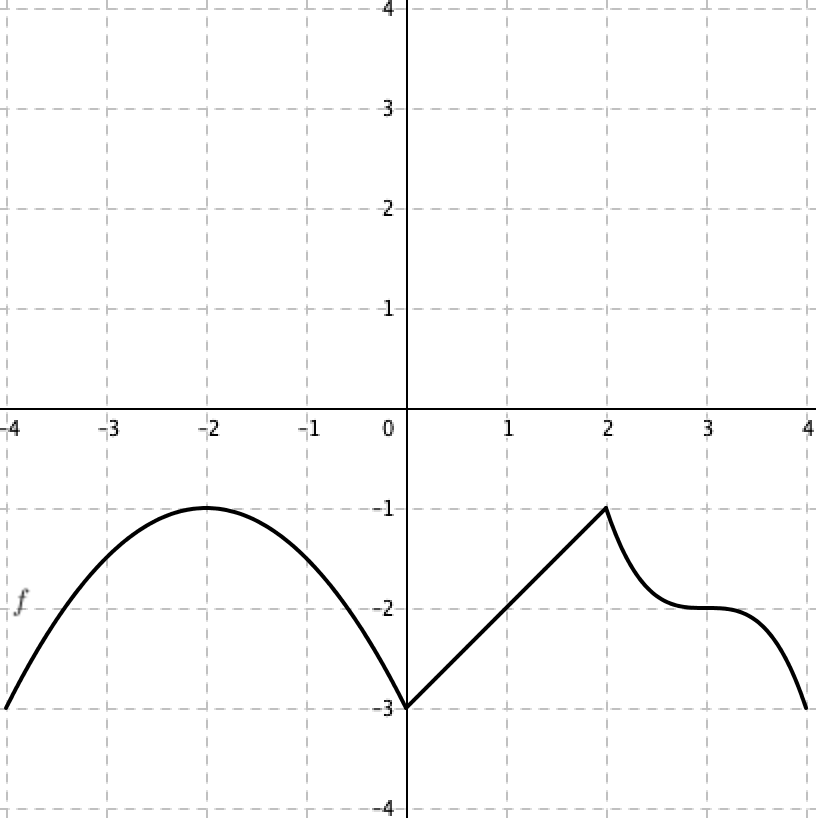
\includegraphics{images/mt2-11_fxn.png}} \hspace{0.25in} \scalebox{0.65}{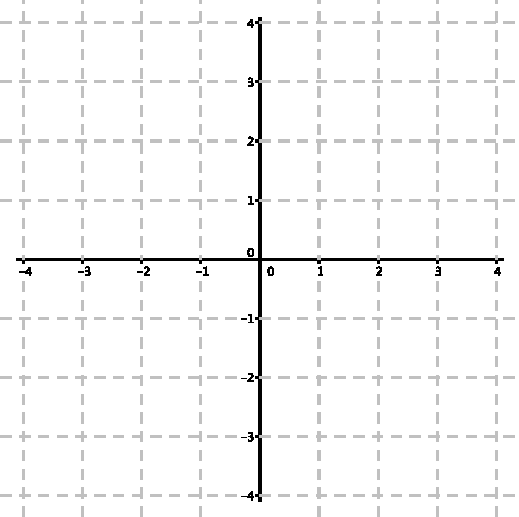
\includegraphics{images/mt2_grid.eps}} \\
\end{center}


	\item % Now make this one tabular and with complicated functions
Consider the two piecewise linear functions $r$ and $s$ given by the figure below.  Determine each of the following derivative values that involve functions that are defined in terms of $r$ and $s$.  Clearly show your work and thinking using proper notation, be sure your values are \emph{exact} in light of the given information, and write one sentence to explain your overall approach.
	
\begin{center}  
\scalebox{0.4}{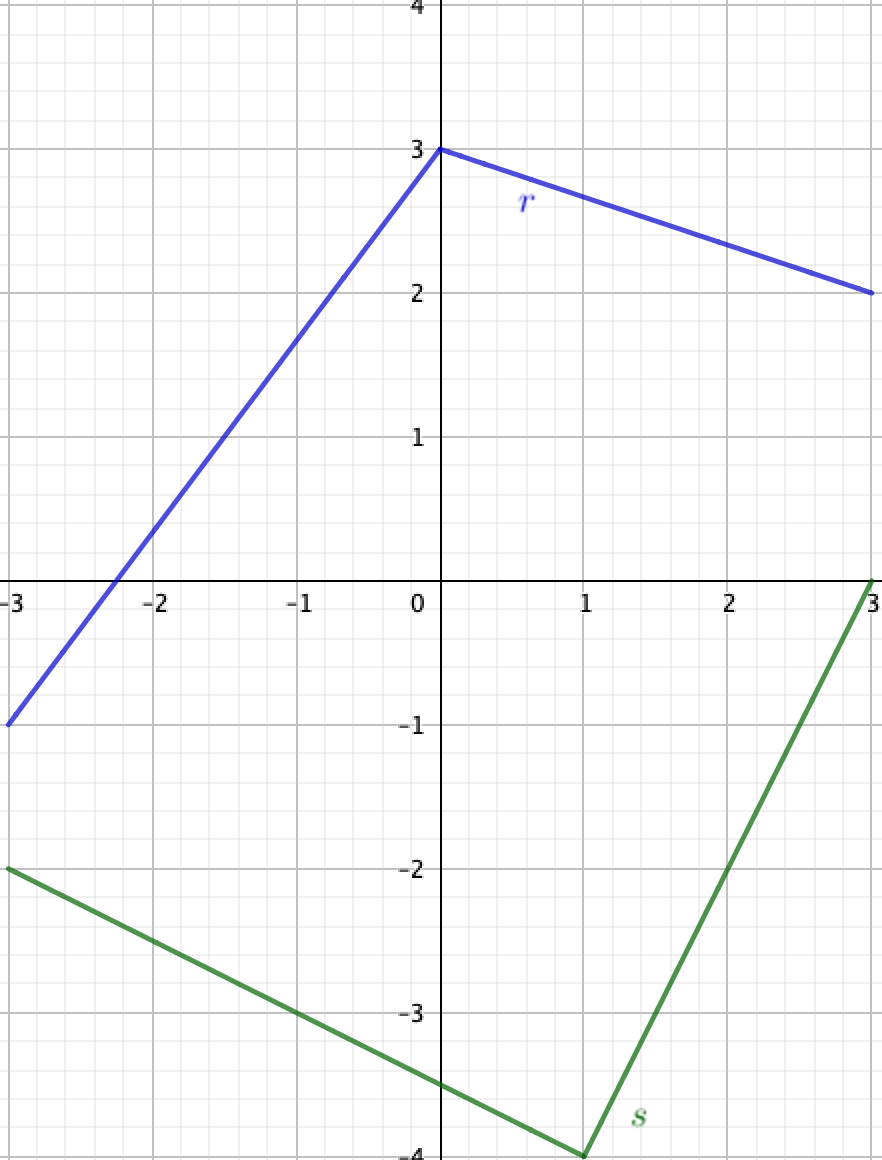
\includegraphics{images/CP7-01-3LTs.png}} \hspace{0.5in} \scalebox{0.6}{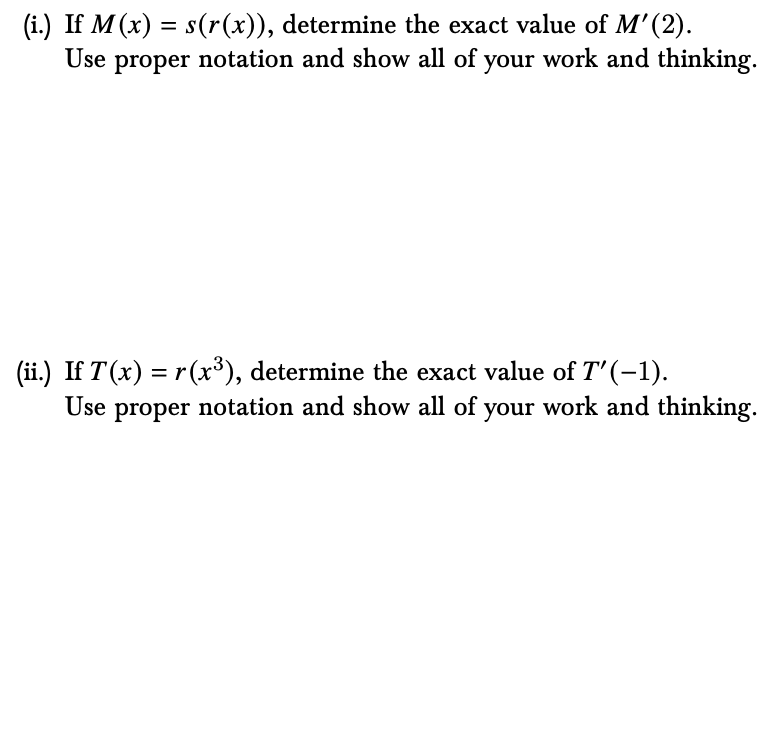
\includegraphics{images/CP3-LT1-chain.png}}
\end{center}


	
%	\be
%		\item[(i.)] If $M(x) = s(r(x))$, determine the exact value of $M'(2)$. \\  
%		Use proper notation and show all of your work and thinking.
%		\lr \tr
%		\item[(ii.)] If $T(x) = r(x^3)$, determine the exact value of $T'(-1)$. \\   
%		Use proper notation and show all of your work and thinking.
%		\lr \tr
%	\ee


%\begin{itemize}
%	\item[(i.)] $N(x) = h(x^3+2x)$.  Determine $N'(-1)$.
%	\lr
%	\item[(ii.)]  Let $R(x) = \sqrt{g(x)}$.  Determine $R'(2)$.
%	\lr
%\end{itemize}	

		\item Evaluate the following definite integral exactly using the Fundamental Theorem of Calculus.  Show your full work and thinking using proper notation.
		
		$\ds \int_{\pi/2}^{\pi} \left(\sin(x) + 2e^x - \frac{1}{x} \right) \, dx$
	\ee

	
	\item[2.] {\bf LT 2}: I can construct an accurate graph of the antiderivative of a function. (Section 5.1)

 Consider the piecewise linear function $y = f(x)$ pictured below; assume that $f(x) = 0$ for $x \le -1$ and $f(x) = 1$ for $x \ge 11$.
	
	\begin{center}
		\scalebox{0.36}{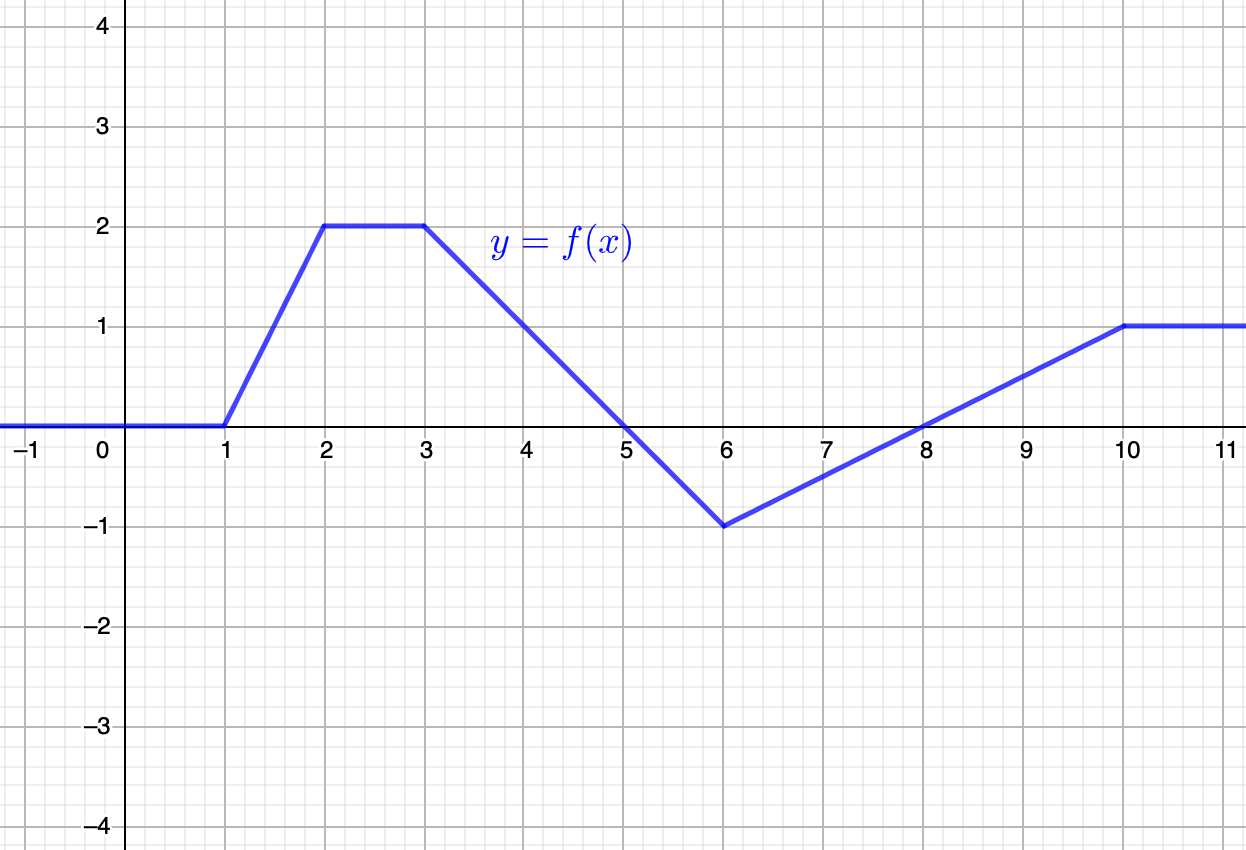
\includegraphics{images/CP-3-LT2-graph.png}} \hspace{0.25in} \scalebox{0.36}{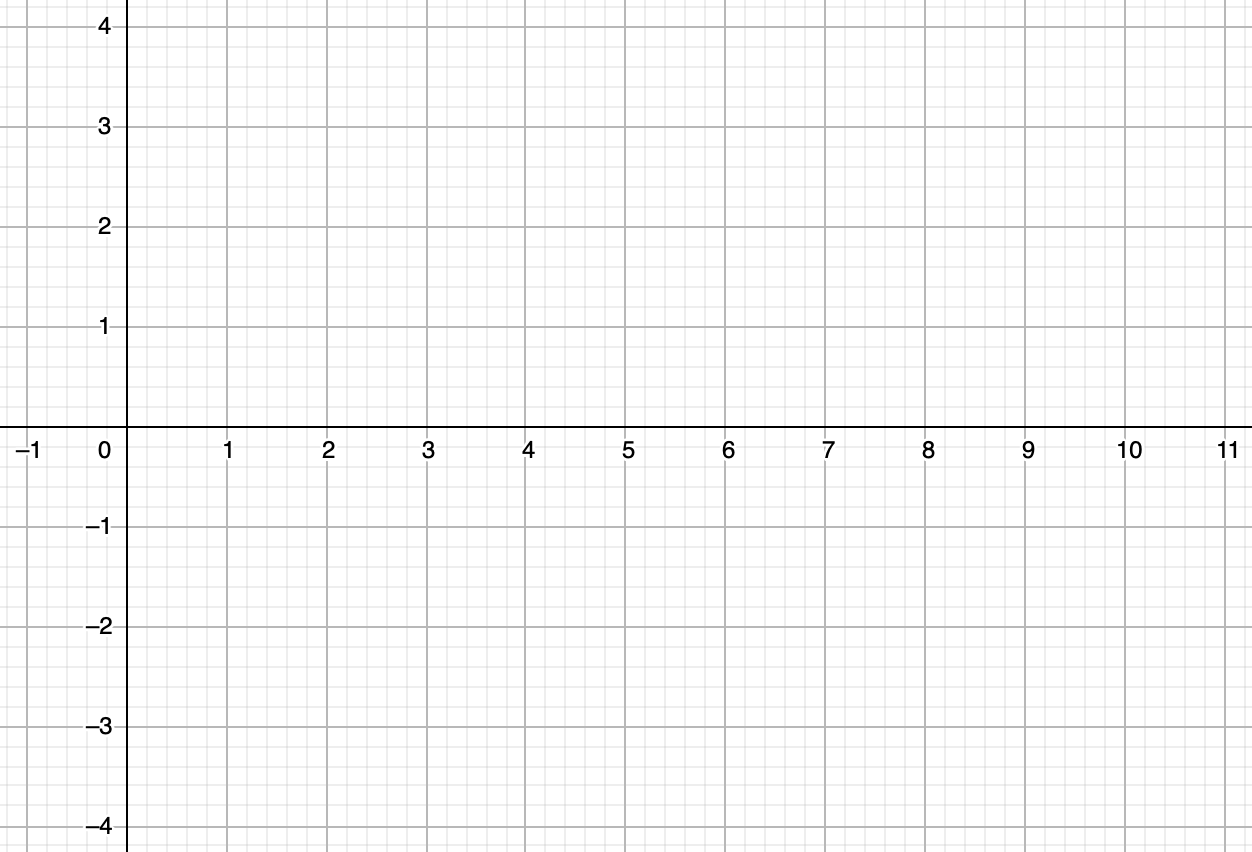
\includegraphics{images/CP-3-LT2-grid.png}} 
	\end{center}
	
	Let $F$ be an antiderivative of $f$ that satisfies $F(1) = -2$.
	
	\be
		\item On what intervals is $F$ increasing?  decreasing? neither?  why?
		
		\item On what intervals is $F$ concave up?  concave down?  neither?  why?
		
		
		\item Find the exact values of $F(2)$, $F(3)$, $F(5)$, $F(6)$, $F(8)$, and $F(10)$.  Write one sentence to explain briefly how you found these values.
		
		\item On the blank grid at right, sketch an accurate, labeled graph of $y = G(x)$.
		
	\ee
	
	\pagebreak


%{\bf LT 3}: I can apply the Second Fundamental Theorem of Calculus to find the antiderivative of a function in terms of an integral and also use the FTC to differentiate an integral function. (Section 5.2)

	\item[3.] {\bf LT 3}: I can apply the Second Fundamental Theorem of Calculus to find the antiderivative of a function in terms of an integral and also use the Second FTC to differentiate an integral function. (Section 5.2)

	\be
		\item State an antiderivative $H$ of the function $\ds h(x) = \frac{10}{3e^{-x/2} + 1}$ that has the property that $H(0) = 2$.  Write one sentence to explain how you determined your formula.
		
		
		\item Suppose that $y = g(x)$ is the piecewise function given by the graph below, and let $G(x) = \int_3^x g(t) \, dt$.
		
	\begin{center}
		\scalebox{0.5}{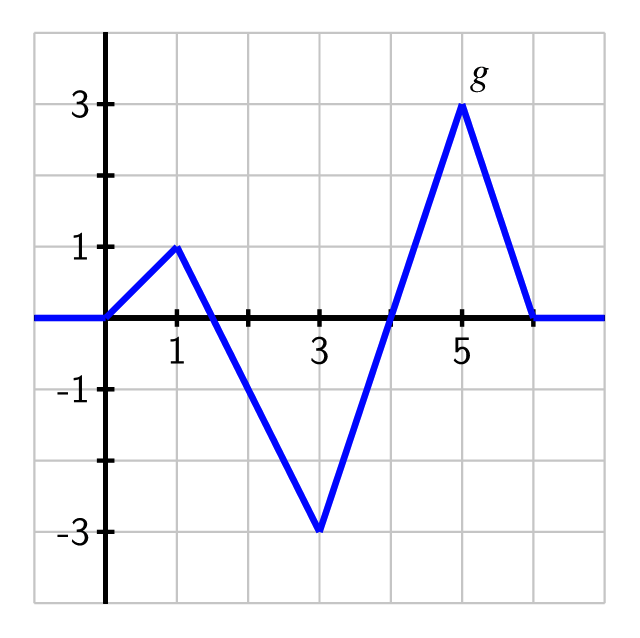
\includegraphics{images/CP-3-LT3-graph.png}} 
	\end{center}
	
		\be
			\item Determine $G'(5)$.  Write briefly to explain how you found its value.
			
			
			\item At what $x$-value(s) is $G'(x) = 0$?  Why?
		\ee
	\ee


\noindent \hrulefill \\


\item[4.] {\bf LT 4}: I can use integration by substitution and integration by parts to evaluate integrals. (Sections 5.3 and 5.4). {\bf Note.} Implicit in this learning target is that you can decide which method to apply to evaluate a given integral and clearly identify the substitution needed to use the method.


	\be
		\item Evaluate each of the following integrals either using $u$-substitution or integration by parts.  For each, \emph{clearly state your substitution/method including any new variables you use, show all of your work, and write one sentence that explains what motivated your choice of method and substitution}.  Your process is even more important than your answer in each.

			\be
			
				\item $\ds \int x^3 \sin(x^4 + 3) \, dx$
			
				
				
				\item $\ds \int 2x e^{2x} \, dx$
			
				
			\ee
	
		\item Consider an integral of the form
		$$\int x^2 \cos(g(x)) \, dx$$

			\be
			
				\item	Give an example of a function you could choose for $g(x)$ that would allow you to evaluate the integral $\int x^2 \cos(g(x)) \, dx$ using $u$-substitution.   State your function $g(x)$ clearly and state the full $u$-substitution you'd use, but {\bf don't} actually evaluate the integral.  \emph{Write a sentence to explain your thinking.}

					
				
				\item Give an example of a function you could choose for $g(x)$ that would allow you to evaluate the integral $\int x^2 \cos(g(x)) \, dx$ using integration by parts.   State your function $g(x)$ clearly and state the full substitution you'd use (that is, state $u$, $du$, $dv$ and $v$, but {\bf don't} actually evaluate the integral.  \emph{Write a sentence to explain your thinking.}
	

				

			\ee
	\ee
	
	\pagebreak

\item[5.] {\bf LT 5}: I can apply an appropriate technique to approximate a definite integral. (Section 5.6)

Suppose we know the following information about a function $g(x)$: $g$ is continuous on the interval $[4,6.4]$, \\ $g$ is either always increasing or always decreasing on the interval, and $g$ is either always concave up or always concave down.  In addition, we have the following data:

	\begin{center}
		\begin{tabular}{l|ccccccccc}
		$x$  & 4.0 & 4.3 & 4.6 & 4.9 & 5.2 & 5.5 & 5.8 & 6.1 & 6.4 \\
		\hline 
		$g(x)$ & -3.0 & -1.8 & -0.8 & 0.05 & 0.6 & 0.95 & 1.2 & 1.1 & 1.06 
		\end{tabular}
	\end{center}

Use the given information to determine the best possible estimate you can for $\ds \int_4^{6.4} g(x) \, dx$. \\  
Start by finding $L_4$, $R_4$, and $M_4$ as estimates of $\ds \int_4^{6.4} g(x) \, dx$, and then use them appropriately to do find the best possible estimate.  \\  

Show a clear summary of your computations using appropriate notation, and write one sentence to explain how you found your final estimate.

\noindent \hrulefill \\


%{\bf LT 6}: I can use definite integrals to find the area between two curves and the volume of a solid of revolution. (Sections 6.1 and 6.2)

\item[6.] {\bf LT 6}: I can use definite integrals to find the area between two curves and the volume of a solid of revolution. (Sections 6.1 and 6.2)

For each of the following prompts, {\bf set up, but do not evaluate, a single definite integral that gives the area or volume of each region described}.  Your processes are even more
important than your final answers here, so show all of your work in a clear and logical order. \emph{For each, include a careful, labeled plot, a representative slice, the area/volume of that representative slice, and make
sure your final answer is clearly indicated (for example by circling it).}
	
	
	\be
		\item The exact area of the finite region bounded by $x = -(y-2)^2$ and $y = x + 6$. \\
		
		\scalebox{0.27}{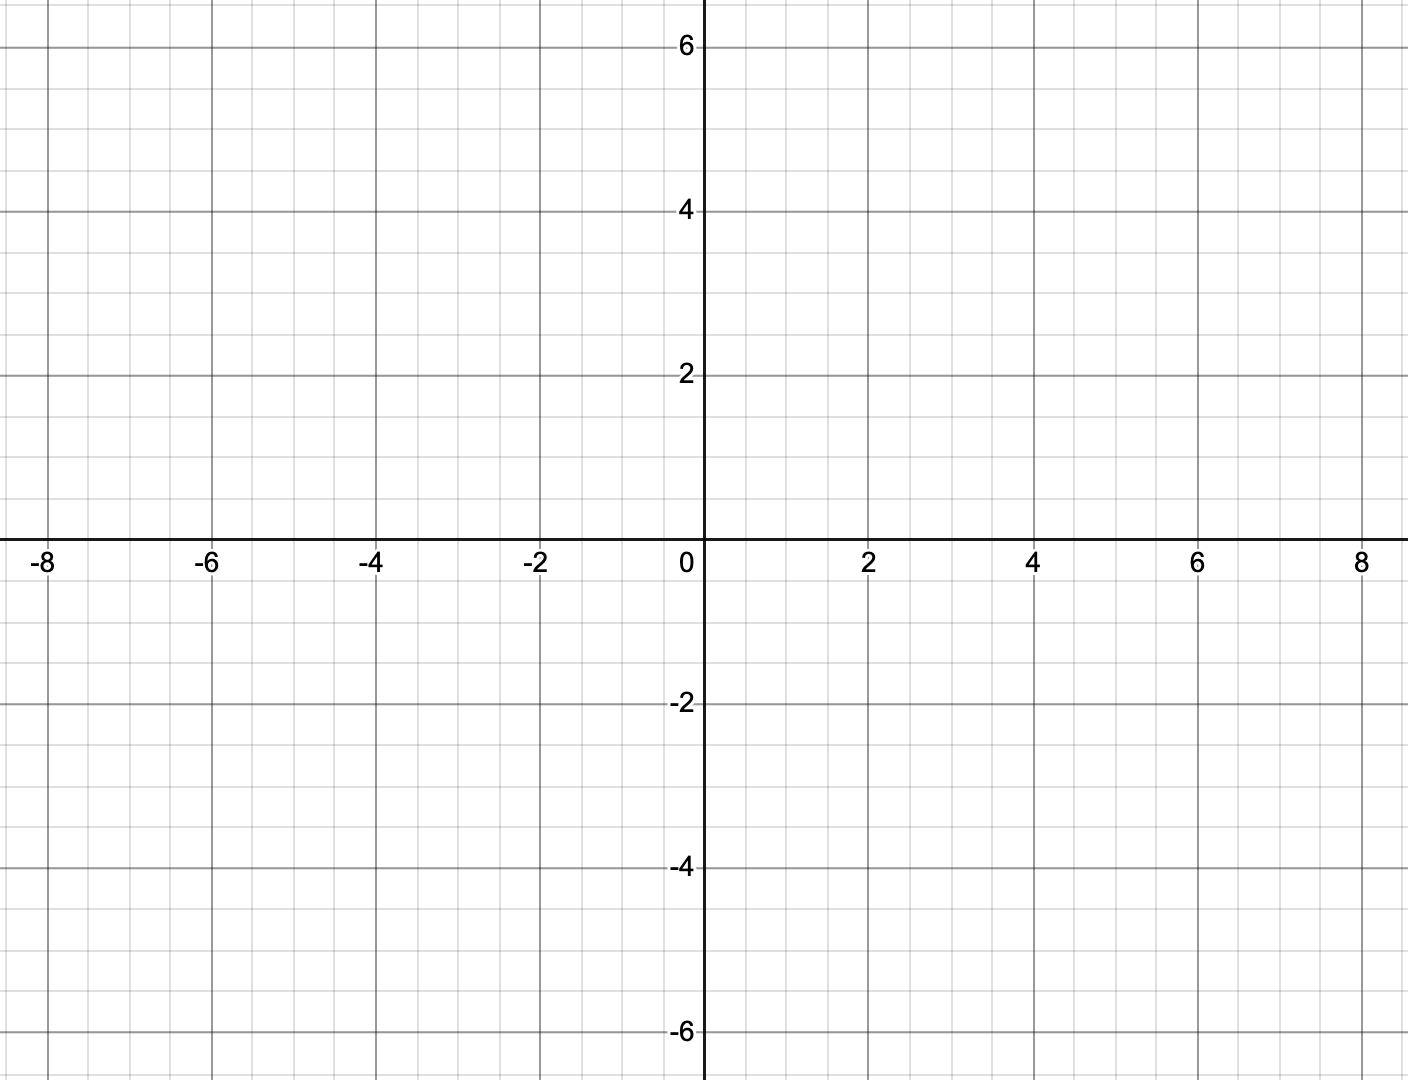
\includegraphics{images/CP-5-blank-grid-LT6.png}} \\
	 	
		\item The exact volume that results from taking the finite region bounded by $y = \frac{1}{2}(x-3)^2+2$ and $x = 5 - y$ and revolving that region about the $x$-axis. \\
		
		\scalebox{0.27}{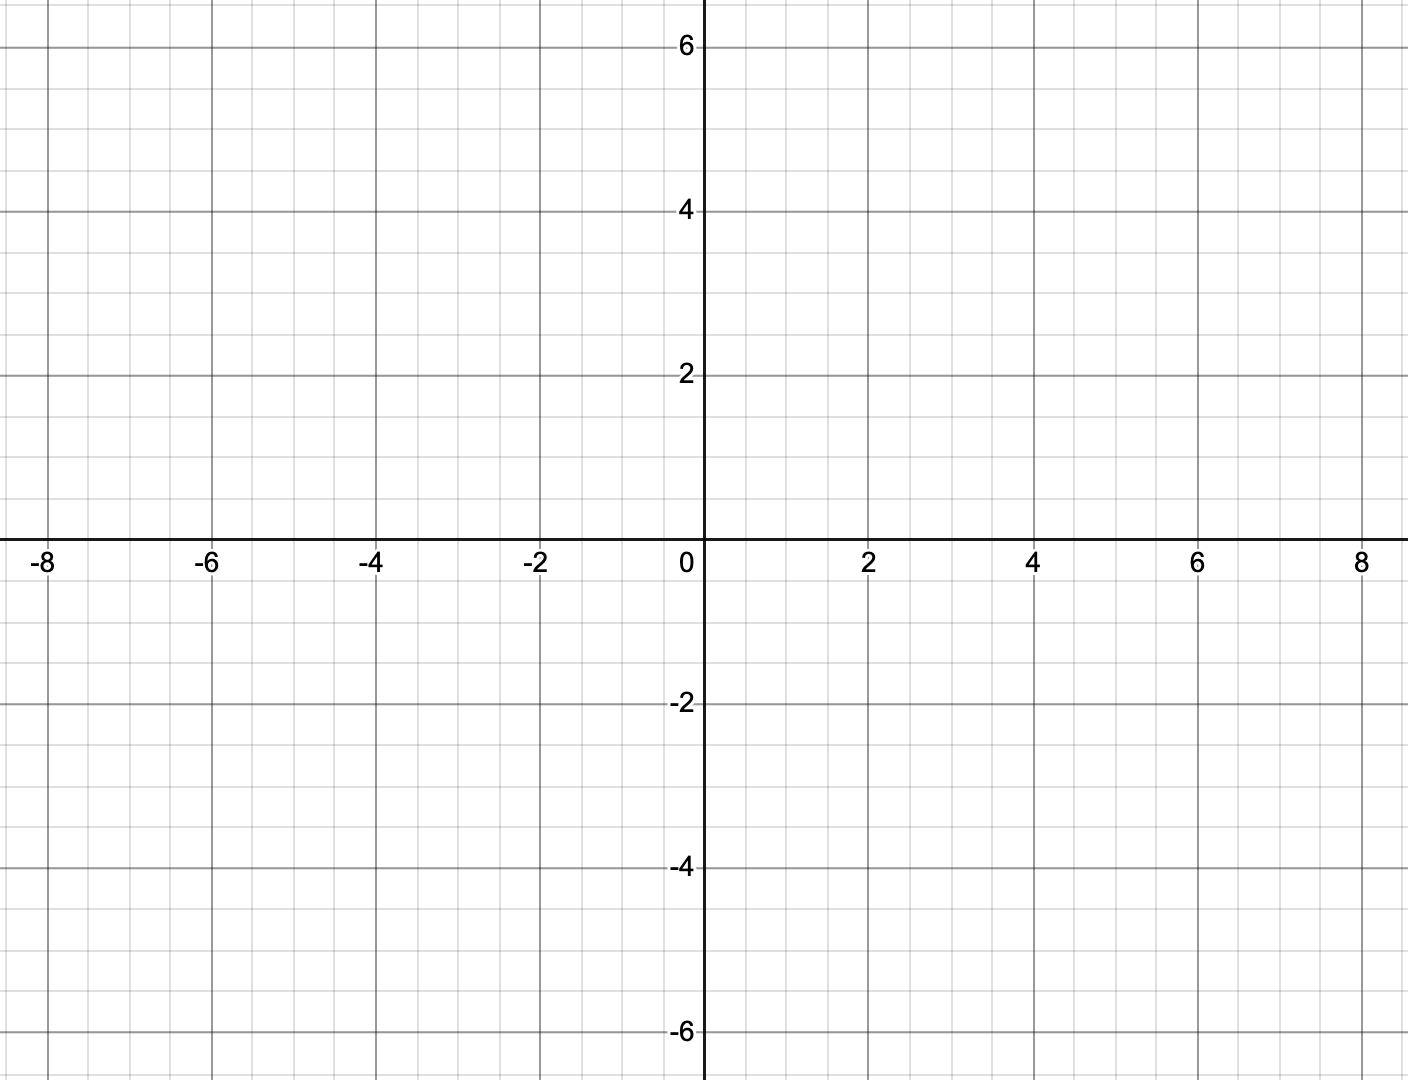
\includegraphics{images/CP-5-blank-grid-LT6.png}} \\
	 	
		\item The exact volume that results from taking the finite region bounded by $y = \frac{1}{2}(x-3)^2+2$ and $x = 5 - y$  and revolving that region about the $y$-axis. \\
		
		\scalebox{0.27}{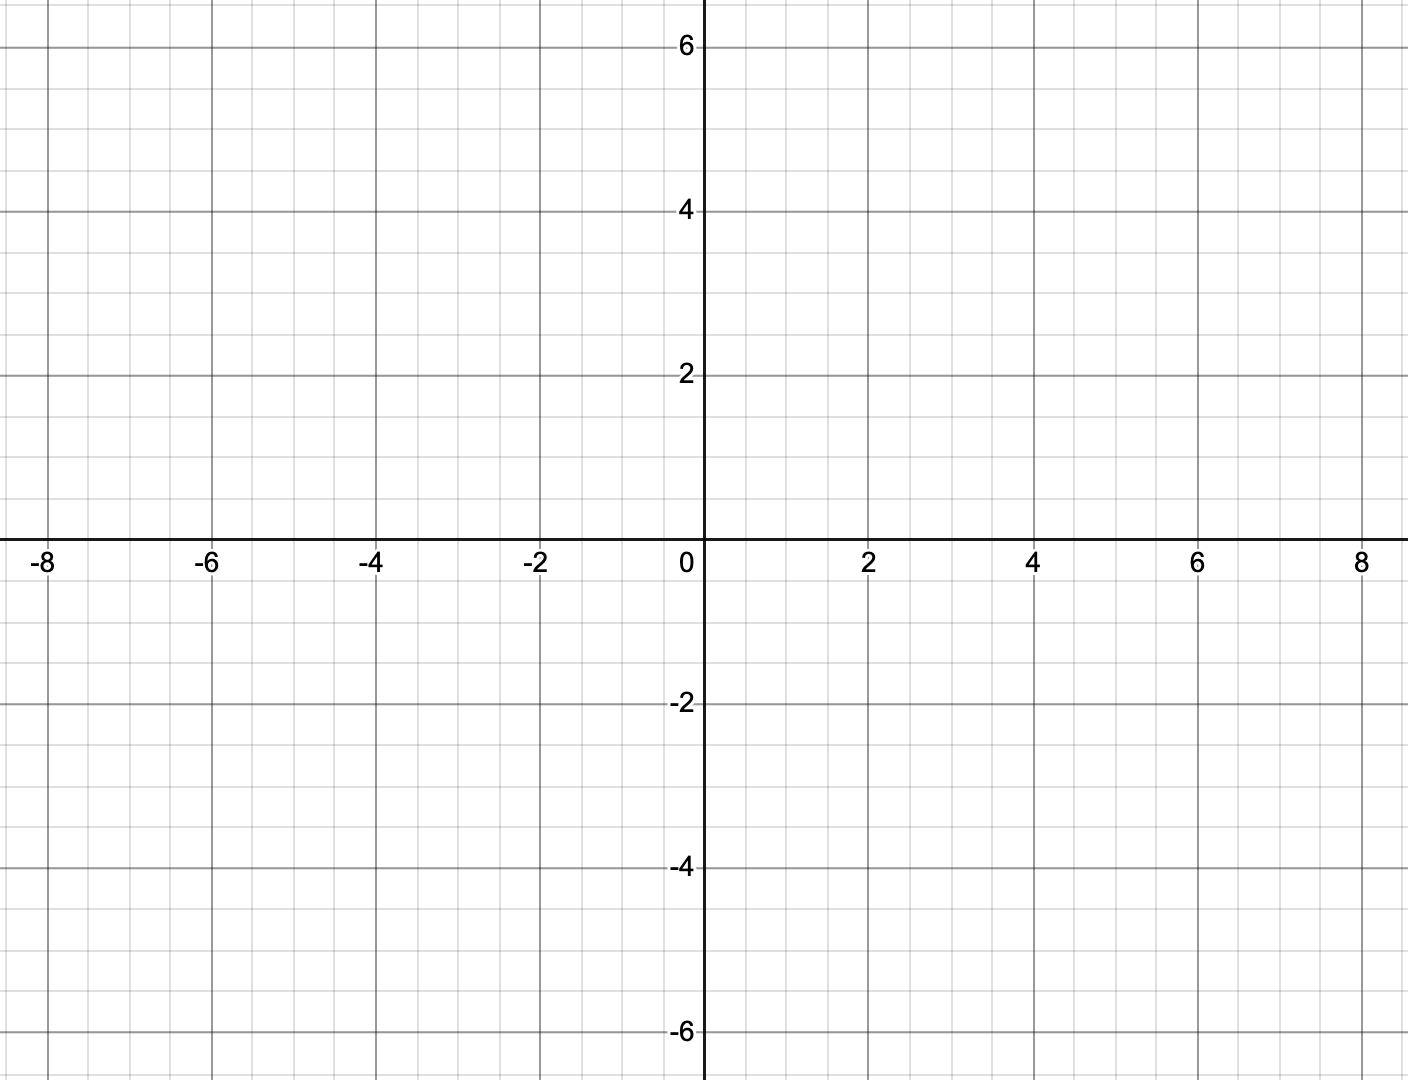
\includegraphics{images/CP-5-blank-grid-LT6.png}} \\		
	\ee


\item[7.]  {\bf LT 7}: I can use definite integrals to find the mass and center of mass of an object.

Let a thin rod with constant cross-sectional area of $1$ cm$^2$ be given.  Assume the rod is 6 cm long and is situated so that its left end lies at $x = 0$ on the horizontal axis.  Suppose that the rod's density is distributed along the rod by the function $\rho(x) = 2e^{-(x-4)^2}$, measured in grams per cm.

	\be
		\item From the graph of $\rho(x)$ (without doing any computations), do you expect the rod's center of mass, $\overline{x}$, to lie at $x = 3$, left of $x = 3$, or right of $x = 3$?  Why?
		
		\item Find the mass $M$ and center of mass $\overline{x}$ by stating appropriate definite integrals and evaluating them using technology.  Clearly identify your results.
		
		\item From the graph of $\rho(x)$ (without doing any computations), how would the rod's mass and center of mass change (if at all) if the density function was instead $\rho(x) = 2e^{-(x-2)^2}$?  Write a sentence to discuss.
		
		\item Returning to the original density function function $\rho(x) = 2e^{-(x-4)^2}$ for the bar of length 6 cm, estimate the value of $a$ for which 90\% of the mass of the bar lies to the left of $a$.  Show a clear summary of your work and thinking. 
	\ee	

\pagebreak

% {\bf LT 8}: I can use definite integrals to represent key quantities in applications such as the work done by a varying force or the pressure that water exerts against a dam. (Section 6.4)

\item[8.] {\bf LT 8}: I can use definite integrals to represent key quantities in applications such as the work done by a varying force or the pressure that water exerts against a dam. (Section 6.4)

Consider a trough with a triangular end as pictured below.  

%Assume the trough is 16 feet wide along its top, 20 feet deep, 30 feet long, and that it is full of water to a depth of 17 feet.   As usual, the weight density of water is 62.4 pounds per cubic foot.

Assume the trough is 12 feet wide along its top, 15 feet deep, 18 feet long, and that it is full of water to a depth of 13 feet.   As usual, the weight density of water is 62.4 pounds per cubic foot.

\be

	\item \emph{Determine the total amount of hydrostatic force on one end of the trough}.  Clearly show relevant slices that go in to determining the definite integral that answers the question. State the appropriate definite integral clearly and evaluate it using technology to determine the total work to achieve the task noted above.  Include units on your result.

\hfill \scalebox{0.4}{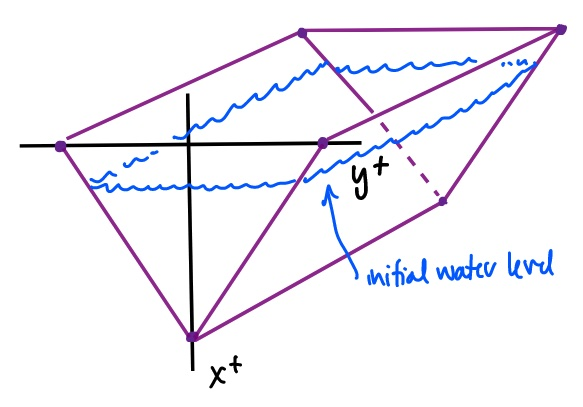
\includegraphics{images/LT-8-tank-3}}


%v1 - Determine the total amount of work that would be required to empty the tank until 4 feet of water remains in it, while pumping the water to a truck whose tank is 2 feet above the top of the tank}

%v2 - Determine the total amount of work that would be required to empty the tank until 3 feet of water remains in it, while pumping the water to a truck whose tank is 6 feet above the top of the tank}

	\item \emph{Determine the total amount of work that would be required to empty the tank until 3 feet of water remains in it, while pumping the water to a truck whose tank is 6 feet above the top of the tank}.  In your response, clearly show the relevant slice(s) and computations that are involved in determining the definite integral that answers the question.  State the appropriate definite integral clearly and evaluate it using technology to determine the total work to achieve the task noted above.  Include units on your result.
	
\hfill \scalebox{0.4}{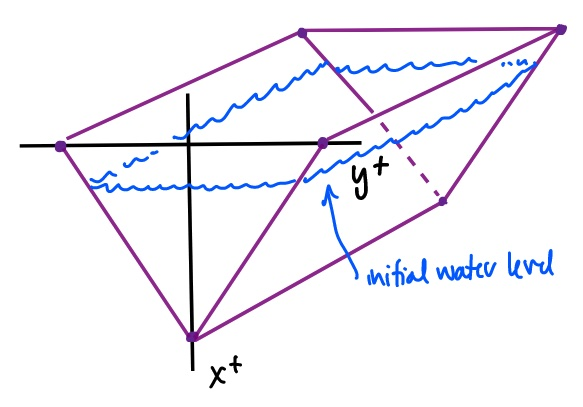
\includegraphics{images/LT-8-tank-3}}

\ee  


%{\bf LT 10}: I can check whether a function is a solution to a differential equation and explain why the function is or is not a solution.

\item[9.] {\bf LT 9}: I can check whether a function is a solution to a differential equation and explain why the function is or is not a solution.  (Section 7.1)

For each of the following prompts, determine whether or not the given function is or is not a solution to the given differential equation.  For each, show your computational/algebraic work and write a brief sentence to clearly justify your conclusion.
	
	
	\be
		\item $\frac{dM}{dt} = 0.1M - 10$, $M(t) = 100 + 5e^{0.1t}$
		%$y(t) = \frac{1}{3}t^3 + e^{2t} + 5$; $\frac{dy}{dt} = t^2 + e^{2t}$		

	
		\item $\frac{dQ}{dt} = -4Q$, $Q(t) = \sin(4t)$
		%$P(t) = 4$; $\frac{dP}{dt} = -3P(4-P)$
		
		
		\item $\frac{dy}{dt} = -4t$, $y(t) = -2t^2 + 11$
		%$F(t) = 70 + 25e^{-0.1t}$; $\frac{dF}{dt} = -\frac{1}{10}F  + 7$
		
		
		\item $\frac{dP}{dt} = -0.05 P (20 - P)$, $P(t) = 20$
		%$A(t) = \cos(2t)$; $\frac{dA}{dt} = -2A$
		
		

	\ee


\item[10.] {\bf LT 10}:  I can apply Euler’s Method to generate an approximate solution to an initial value problem and explain the result’s meaning in context. (Section 7.3)

Consider the initial value problem $\frac{dy}{dx} = 0.25x + 0.5y$, $y(0) = -1$.

Apply Euler's Method with $\Delta x = 0.25$ to estimate $y(0.75)$.  

Clearly show your work and thinking below (that is, show how at least one row in your table is determined), and fill in the given table accordingly (there are more rows in the table than you'll need; you decide how many rows you need).  Write at least one sentence to summarize your work and your final answer to the main question posed.


\begin{center}
\begin{tabular}{|c|c|c|c|c|}
\hline
$\Delta x$ & $x$ & $y$ &  Slope   &  $\Delta y$ \\
\hline
  \ \hspace{0.5in} \ & \ \hspace{0.5in} \  & \ \hspace{0.5in} \  & \  \hspace{0.5in} \ & \  \hspace{0.5in} \ \\   \hline  
  \ & \ & \ & \ & \ \\ \hline
    \ & \ & \ & \ & \ \\  \hline
  \ & \ & \ & \ & \ \\  \hline
   \ & \ & \ & \ & \ \\   \hline
   \ & \ & \ & \ & \ \\   \hline   
   \ & \ & \ & \ & \ \\  
\hline
\end{tabular}
\end{center}


%{\bf LT 12}:  I can express real world situations as differential equations, determine any stable or unstable equilibrium solutions, and explain the significance of the equilibrium solutions in context. (Section 7.5)

% do a mixing problem

\item[11.] {\bf LT 11}:  I can express real world situations as differential equations, determine any stable or unstable equilibrium solutions, and explain the significance of the equilibrium solutions in context. (Section 7.5)

\be
	\item Say that you have an investment account that has a principal amount that earns interest, plus you withdraw a fixed amount annually.  In particular, suppose that you have \$$M(t)$  in the account at time $t$ in years; that the account earns 5\% interest compounded continuously; and that you withdraw \$1000  once a year.  Suppose that initially you have $M(0) = 50,000$ in the account.
	
	\be
		\item Set up an initial value problem whose solution is $M(t)$.  Write to demonstrate your thinking behind the various parts of your differential equation.
		
		\item What is the equilibrium solution to the differential equation you determined?  Why does this make sense in terms of the physical reality of money?  Explain.
		
	\ee
	
	
	\item Suppose that biologists are studying the trout population in the Muskegon river, and they observe that due to natural death and harvesting by people who catch and keep fish, the trout population is actually decreasing at a rate proportional to itself.  That is, if the population of trout is $F(t)$ in year $t$, then the rate of change of $F$ is proportional to $F$ with proportionality constant $k = -0.025$.  
	
	\be
		\item Set up a differential equation whose solution is $F(t)$.  Write to demonstrate your thinking.
		
		\item Now suppose that in order to prevent the fish population from dying out, the Michigan DNR plants 20,000 fish in the river each year.  Set up a new differential equation -- one that builds upon your work in (i) and that also takes into account this annual addition of fish to the system -- whose solution is $F(t)$.
		
		\item What is the equilibrium solution to the updated differential equation in (b)-(ii)?
	\ee
	
	
\ee


	\end{enumerate}
	
\end{document}

